\subsection{Simplified Memory Addressing}
\label{subsec:simple-address}

Indirect memory operations in OE require the mapped program to form and update
matrix addresses during execution. We estimate the cycle cost of simplifying
this mechanism by replacing matrix loads and stores with column-shared direct
access pointers that advance by one word. Before each run, Python arranges the
operands into four column-specific sequential streams and maps the output
streams back to the conventional matrix layout. All arithmetic, including
$\alpha AB+\beta C$ in GEM, remains on the CGRA. The preparation pass traces
the original access schedule and its time and memory are excluded from kernel
cycles.

Table~\ref{tab:simple-address-cycles} reports the simulated cycles. The
direct-access streams reproduced every indirect load value and store address,
and all outputs matched an independent CPU reference exactly. Simplified
addressing removes two address-generation PCs from MMUL and four from GEM;
remaining PCs retain loop-counter propagation and branch control. The
percentage reduction falls with matrix size because the unchanged arithmetic
dominates larger runs. GEM benefits more because its schedule contains two
additional removable address PCs.

\begin{table}[t]
\centering
\caption{Simulated cycles and speedup for simplified memory addressing.}
\label{tab:simple-address-cycles}
\begin{tabular}{lrrrrr}
\hline
Kernel & Size & OE original & Simple Address & Reduction & Speedup \\
\hline
MMUL & $16\times16$ & 4,644 & 4,564 & 1.72\% & 1.018$\times$ \\
MMUL & $32\times32$ & 34,584 & 34,304 & 0.81\% & 1.008$\times$ \\
MMUL & $64\times64$ & 268,992 & 267,928 & 0.40\% & 1.004$\times$ \\
MMUL & $128\times128$ & 2,124,048 & 2,119,880 & 0.20\% & 1.002$\times$ \\
GEM & $16\times16$ & 5,543 & 5,423 & 2.16\% & 1.022$\times$ \\
GEM & $32\times32$ & 38,075 & 37,659 & 1.09\% & 1.011$\times$ \\
GEM & $64\times64$ & 282,851 & 281,267 & 0.56\% & 1.006$\times$ \\
GEM & $128\times128$ & 2,179,379 & 2,173,155 & 0.29\% & 1.003$\times$ \\
\hline
\end{tabular}
\end{table}

\begin{figure}[t]
\centering
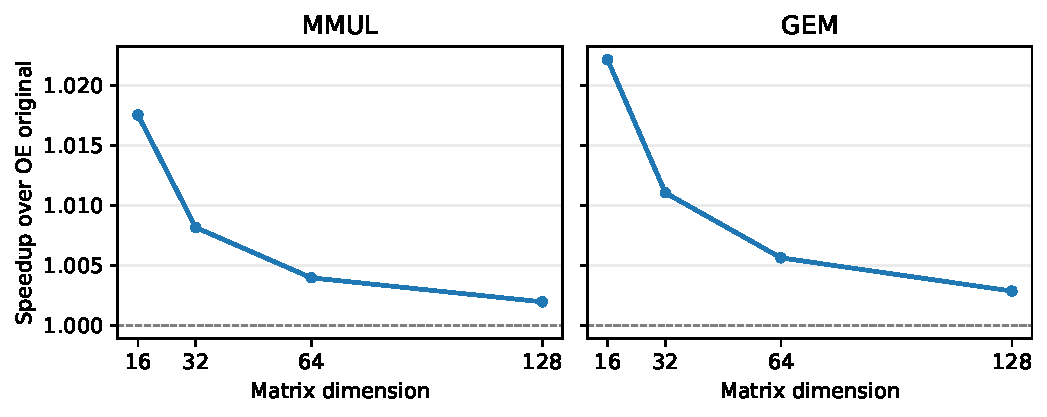
\includegraphics[width=0.92\linewidth]{benchmarks/DISCOvsOE/simple_address_speedup.pdf}
\caption{Speedup of the sequential direct-address layout over the original
indirect-address kernels.}
\label{fig:simple-address-speedup}
\end{figure}

This cycle reduction trades run-time address work for substantial
preconfiguration. Counting each memory element as one 32-bit word, the
prepared layout grows from 2.94$\times$ to 21.66$\times$ the original MMUL
storage and from 3.25$\times$ to 21.99$\times$ for GEM as dimensions increase
from 16 to 128. At 128, the streams repeat 1,015,808 values; Python
preparation, including schedule tracing, takes about 25--26 seconds. These
results characterize an idealized data-layout transformation in the
simulator, not a physical-memory implementation or an end-to-end speedup.
